\documentclass{standalone}
\usepackage{tikz}
\usetikzlibrary{patterns, positioning}

\begin{document}
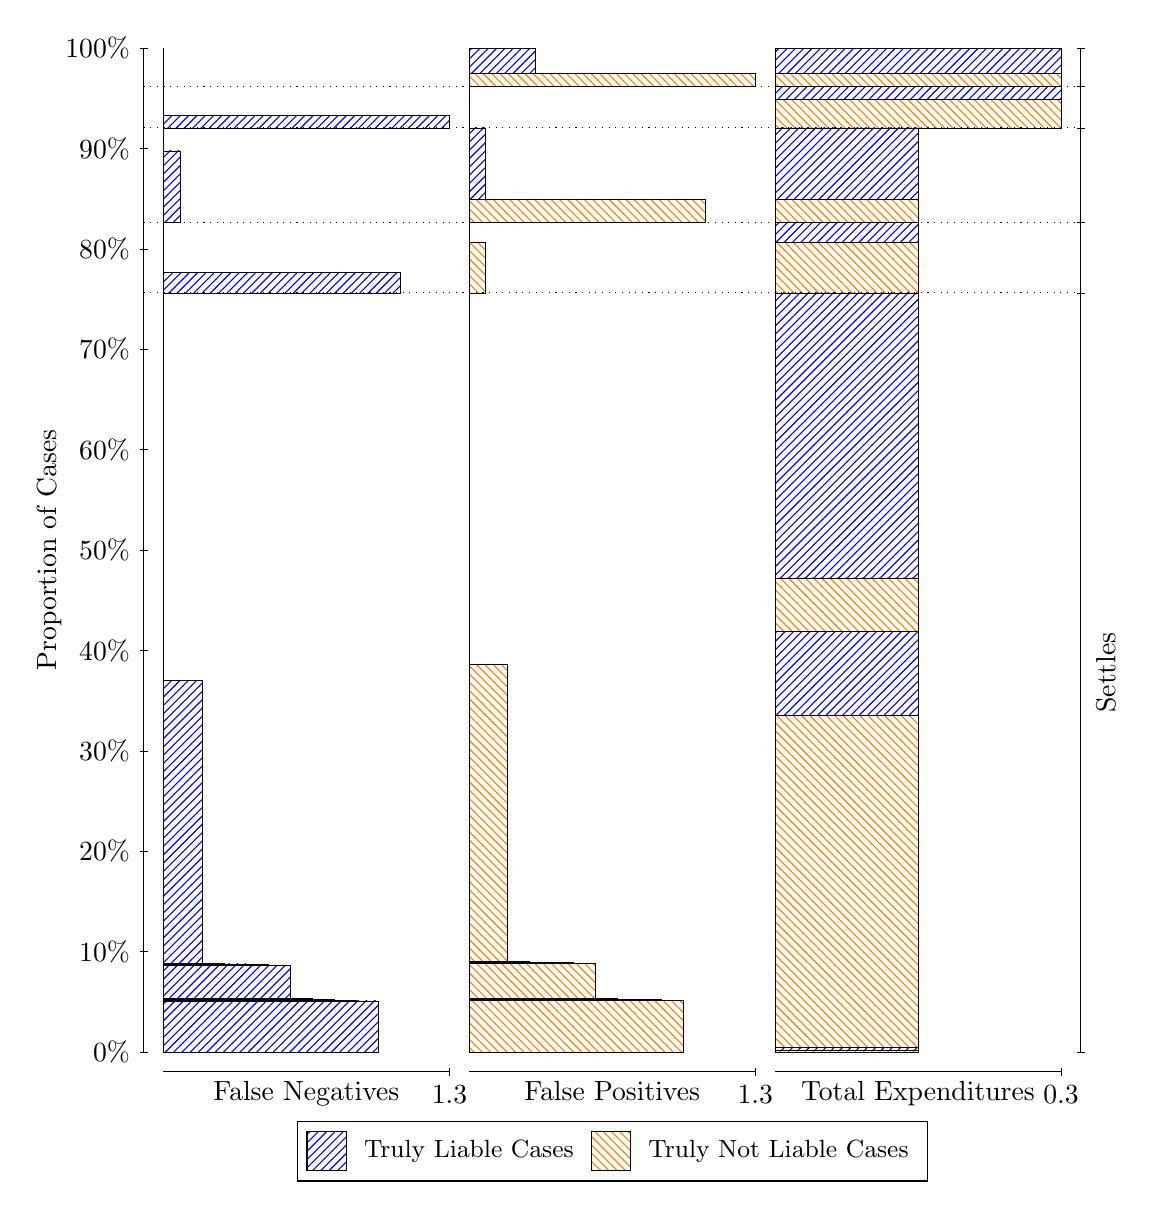
\begin{tikzpicture}
\draw[black, very thin] (1.5,1.75) -- (1.5,14.5);
\node[rotate=90, anchor=center] at (0.3, 8.125) {Proportion of Cases};
\draw[black, very thin] (1.45,1.75) -- (1.55,1.75);
\node[anchor=east] at (1.45, 1.75) {0\%};
\draw[black, very thin] (1.45,3.025) -- (1.55,3.025);
\node[anchor=east] at (1.45, 3.025) {10\%};
\draw[black, very thin] (1.45,4.3) -- (1.55,4.3);
\node[anchor=east] at (1.45, 4.3) {20\%};
\draw[black, very thin] (1.45,5.575) -- (1.55,5.575);
\node[anchor=east] at (1.45, 5.575) {30\%};
\draw[black, very thin] (1.45,6.85) -- (1.55,6.85);
\node[anchor=east] at (1.45, 6.85) {40\%};
\draw[black, very thin] (1.45,8.125) -- (1.55,8.125);
\node[anchor=east] at (1.45, 8.125) {50\%};
\draw[black, very thin] (1.45,9.4) -- (1.55,9.4);
\node[anchor=east] at (1.45, 9.4) {60\%};
\draw[black, very thin] (1.45,10.675) -- (1.55,10.675);
\node[anchor=east] at (1.45, 10.675) {70\%};
\draw[black, very thin] (1.45,11.95) -- (1.55,11.95);
\node[anchor=east] at (1.45, 11.95) {80\%};
\draw[black, very thin] (1.45,13.225) -- (1.55,13.225);
\node[anchor=east] at (1.45, 13.225) {90\%};
\draw[black, very thin] (1.45,14.5) -- (1.55,14.5);
\node[anchor=east] at (1.45, 14.5) {100\%};

\draw[black, very thin] (13.4,1.75) -- (13.4,14.5);
\draw[black, very thin] (13.35,1.75) -- (13.45,1.75);
\node[anchor=west] at (13.35, 1.75) {};
\draw[black, very thin] (13.35,11.39) -- (13.45,11.39);
\node[anchor=west] at (13.35, 11.39) {};
\draw[black, very thin] (13.35,12.284) -- (13.45,12.284);
\node[anchor=west] at (13.35, 12.284) {};
\draw[black, very thin] (13.35,13.486) -- (13.45,13.486);
\node[anchor=west] at (13.35, 13.486) {};
\draw[black, very thin] (13.35,14.01) -- (13.45,14.01);
\node[anchor=west] at (13.35, 14.01) {};
\draw[black, very thin] (13.35,14.5) -- (13.45,14.5);
\node[anchor=west] at (13.35, 14.5) {};

\draw[black, very thin, pattern color=blue, pattern=north east lines] (1.75,1.75) rectangle (4.475,2.3985);
\draw[black, very thin, pattern color=blue, pattern=north east lines] (1.75,2.3985) rectangle (4.1955,2.4097);
\draw[black, very thin, pattern color=blue, pattern=north east lines] (1.75,2.4097) rectangle (3.916,2.4213);
\draw[black, very thin, pattern color=blue, pattern=north east lines] (1.75,2.4213) rectangle (3.6365,2.4332);
\draw[black, very thin, pattern color=blue, pattern=north east lines] (1.75,2.4332) rectangle (3.3571,2.852);
\draw[black, very thin, pattern color=blue, pattern=north east lines] (1.75,2.852) rectangle (3.0776,2.86);
\draw[black, very thin, pattern color=blue, pattern=north east lines] (1.75,2.86) rectangle (2.7981,2.8678);
\draw[black, very thin, pattern color=blue, pattern=north east lines] (1.75,2.8678) rectangle (2.5186,2.8754);
\draw[black, very thin, pattern color=blue, pattern=north east lines] (1.75,2.8754) rectangle (2.2391,6.471);
\draw[black, very thin, pattern color=orange, pattern=north west lines] (1.75,6.471) rectangle (1.75,11.39);
\draw[black, very thin, pattern color=blue, pattern=north east lines] (1.75,11.39) rectangle (4.7545,11.646);
\draw[black, very thin, pattern color=orange, pattern=north west lines] (1.75,11.646) rectangle (1.75,12.284);
\draw[black, very thin, pattern color=blue, pattern=north east lines] (1.75,12.284) rectangle (1.9596,13.193);
\draw[black, very thin, pattern color=orange, pattern=north west lines] (1.75,13.193) rectangle (1.75,13.486);
\draw[black, very thin, pattern color=blue, pattern=north east lines] (1.75,13.486) rectangle (5.3833,13.649);
\draw[black, very thin, pattern color=orange, pattern=north west lines] (1.75,13.649) rectangle (1.75,14.01);
\draw[black, very thin, pattern color=orange, pattern=north west lines] (1.75,14.01) rectangle (1.75,14.173);
\draw[black, very thin, pattern color=blue, pattern=north east lines] (1.75,14.173) rectangle (1.75,14.5);
\draw[black, very thin, pattern color=orange, pattern=north west lines] (5.6333,1.75) rectangle (8.3583,2.4051);
\draw[black, very thin, pattern color=orange, pattern=north west lines] (5.6333,2.4051) rectangle (8.0788,2.4137);
\draw[black, very thin, pattern color=orange, pattern=north west lines] (5.6333,2.4137) rectangle (7.7994,2.4225);
\draw[black, very thin, pattern color=orange, pattern=north west lines] (5.6333,2.4225) rectangle (7.5199,2.4315);
\draw[black, very thin, pattern color=orange, pattern=north west lines] (5.6333,2.4315) rectangle (7.2404,2.8759);
\draw[black, very thin, pattern color=orange, pattern=north west lines] (5.6333,2.8759) rectangle (6.9609,2.8761);
\draw[black, very thin, pattern color=orange, pattern=north west lines] (5.6333,2.8761) rectangle (6.9609,2.8842);
\draw[black, very thin, pattern color=orange, pattern=north west lines] (5.6333,2.8842) rectangle (6.6814,2.8922);
\draw[black, very thin, pattern color=orange, pattern=north west lines] (5.6333,2.8922) rectangle (6.4019,2.8999);
\draw[black, very thin, pattern color=orange, pattern=north west lines] (5.6333,2.8999) rectangle (6.1224,6.6694);
\draw[black, very thin, pattern color=blue, pattern=north east lines] (5.6333,6.6694) rectangle (5.6333,11.39);
\draw[black, very thin, pattern color=orange, pattern=north west lines] (5.6333,11.39) rectangle (5.8429,12.029);
\draw[black, very thin, pattern color=blue, pattern=north east lines] (5.6333,12.029) rectangle (5.6333,12.284);
\draw[black, very thin, pattern color=orange, pattern=north west lines] (5.6333,12.284) rectangle (8.6378,12.577);
\draw[black, very thin, pattern color=blue, pattern=north east lines] (5.6333,12.577) rectangle (5.8429,13.486);
\draw[black, very thin, pattern color=orange, pattern=north west lines] (5.6333,13.486) rectangle (5.6333,13.846);
\draw[black, very thin, pattern color=blue, pattern=north east lines] (5.6333,13.846) rectangle (5.6333,14.01);
\draw[black, very thin, pattern color=orange, pattern=north west lines] (5.6333,14.01) rectangle (9.2667,14.173);
\draw[black, very thin, pattern color=blue, pattern=north east lines] (5.6333,14.173) rectangle (6.4718,14.5);
\draw[black, very thin, pattern color=orange, pattern=north west lines] (9.5167,1.75) rectangle (11.333,1.774);
\draw[black, very thin, pattern color=blue, pattern=north east lines] (9.5167,1.774) rectangle (11.333,1.8086);
\draw[black, very thin, pattern color=orange, pattern=north west lines] (9.5167,1.8086) rectangle (11.333,6.0225);
\draw[black, very thin, pattern color=blue, pattern=north east lines] (9.5167,6.0225) rectangle (11.333,7.0899);
\draw[black, very thin, pattern color=orange, pattern=north west lines] (9.5167,7.0899) rectangle (11.333,7.7714);
\draw[black, very thin, pattern color=blue, pattern=north east lines] (9.5167,7.7714) rectangle (11.333,11.39);
\draw[black, very thin, pattern color=orange, pattern=north west lines] (9.5167,11.39) rectangle (11.333,12.029);
\draw[black, very thin, pattern color=blue, pattern=north east lines] (9.5167,12.029) rectangle (11.333,12.284);
\draw[black, very thin, pattern color=orange, pattern=north west lines] (9.5167,12.284) rectangle (11.333,12.577);
\draw[black, very thin, pattern color=blue, pattern=north east lines] (9.5167,12.577) rectangle (11.333,13.486);
\draw[black, very thin, pattern color=orange, pattern=north west lines] (9.5167,13.486) rectangle (13.15,13.846);
\draw[black, very thin, pattern color=blue, pattern=north east lines] (9.5167,13.846) rectangle (13.15,14.01);
\draw[black, very thin, pattern color=orange, pattern=north west lines] (9.5167,14.01) rectangle (13.15,14.173);
\draw[black, very thin, pattern color=blue, pattern=north east lines] (9.5167,14.173) rectangle (13.15,14.5);
\draw[black, dotted] (1.5,11.39) -- (13.4,11.39);
\draw[black, dotted] (1.5,12.284) -- (13.4,12.284);
\draw[black, dotted] (1.5,13.486) -- (13.4,13.486);
\draw[black, dotted] (1.5,14.01) -- (13.4,14.01);
\draw[black, very thin] (1.75,1.5) -- (5.3833,1.5);
\node[anchor=north] at (3.5667, 1.5) {False Negatives};
\draw[black, very thin] (5.3833,1.45) -- (5.3833,1.55);
\node[anchor=north] at (5.3833, 1.45) {1.3};

\draw[black, very thin] (5.6333,1.5) -- (9.2667,1.5);
\node[anchor=north] at (7.45, 1.5) {False Positives};
\draw[black, very thin] (9.2667,1.45) -- (9.2667,1.55);
\node[anchor=north] at (9.2667, 1.45) {1.3};

\draw[black, very thin] (9.5167,1.5) -- (13.15,1.5);
\node[anchor=north] at (11.333, 1.5) {Total Expenditures};
\draw[black, very thin] (13.15,1.45) -- (13.15,1.55);
\node[anchor=north] at (13.15, 1.45) {0.3};

\node[black, centered, rotate=90] at (13.72, 6.5702) {Settles};





\draw (7.449999999999999,1.5) node[draw=none] (baseCoordinate) {};
\begin{scope}[align=center]
        \matrix[scale=0.5, draw=black, below=0.5cm of baseCoordinate, nodes={draw}, column sep=0.1cm]{
            \node[rectangle, draw, minimum width=0.5cm, minimum height=0.5cm, pattern=north east lines, pattern color=blue] {}; &
            \node[draw=none, font=\small] (B) {Truly Liable Cases}; &
            \node[rectangle, draw, minimum width=0.5cm, minimum height=0.5cm, pattern=north west lines, pattern color=orange] {}; &
            \node[draw=none, font=\small] (B) {Truly Not Liable Cases}; \\
            };
\end{scope}

\end{tikzpicture}
\end{document}